\subsection{Discussion of Study Results}
%\val{Does this section seem too drawn out? I remember in the VoiceScript paper, some reviewers mentioned that our discussion of user evaluation felt like "episodic responses about different system features." I want to avoid that this time and really focus on confirming the design concepts from major findings. The main findings I want to emphasize is that: "our interface indeed makes setup easy"; "our interface adds little overhead during delivery"; "presenters like the real time control"; "content affects the choice of interface" (our interface is especially good for process-driven content that is ).}
%\wil{I think it is well-organized, and even if it could be tightened a bit, I prefer to err on the side of completeness at this point. However, it would be useful to include a graph summarizing the ratings. It could be a single graph with 9 individual boxplots for the three questions. We could also show one graph with the votes from Study 2; again, 9 bars in total to cover the three content types.}

Overall, presenters found \interface\ easy to use for setting up and delivering presentations. They were satisfied with the quality of the presentations recorded using our interface, and emphasized that the appearance of real time inking had an engaging effect. 
Preferences between the presentation tools depended on the content type. Participants in both studies (i.e., presenters and viewers) preferred \interface\ for text-centered or process-driven content. 
%
Given the size and exploratory nature of our study, we use descriptive statistics to summarize the Likert responses from Study 1 (Figure~\ref{fig:likert}).
%
Figure~\ref{fig:votes} shows the preference data across content types from both studies.
%
Below we discuss each of our findings in more detail. 

\begin{figure}[t!]
    \centering
        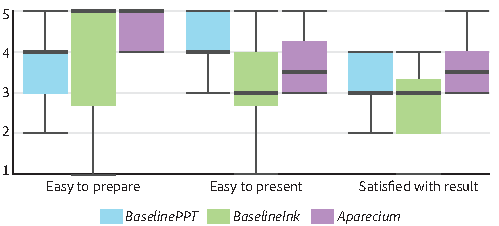
\includegraphics[width=1\columnwidth]{figures/study1likert}
        \caption{Summary of Likert responses from Study 1 on a scale from 1 (strongly disagree) to 5 (strongly agree).}
\label{fig:likert}
\end{figure}

%\definecolor{color1}{rgb}{0.92, 0.83, 0.78}
%\definecolor{color2}{rgb}{0.91, 0.66, 0.66}
%\definecolor{color3}{rgb}{0.68, 0.68, 0.96}
%\begin{figure}
%\centering
%\begin{tikzpicture}
%\begin{axis}[
%ybar,
%enlargelimits=0.15,
%enlarge y limits={upper=0},
%legend style={at={(0.5,-0.15)},
%  anchor=north,legend columns=-1},
%symbolic x coords={Easy Setup, Easy Delivery, Satisfaction},
%xtick=data,
%%    nodes near coords,
%%    nodes near coords align={vertical},
%scaled y ticks = false,
%ymin =0,
%ylabel={Score},
%]
%\addplot[style={fill=color1}, error bars/.cd, y dir=both, y explicit]
%coordinates {
%(Easy Setup, 3.6) += (0,1.0) -= (0,1.0)
%(Easy Delivery, 4.2) += (0,0.7) -= (0,0.7)
%(Satisfaction, 3.3)+= (0,0.8) -= (0,0.8)};
%\addplot[style={fill=color2}, error bars/.cd, y dir=both, y explicit] 
%coordinates {(Easy Setup, 3.9) += (0,0.2) -= (0,0.1)
%(Easy Delivery, 3.3) += (0,0.2) -= (0,0.1)
%(Satisfaction, 2.8)+= (0,0.2) -= (0,0.1)};
%\addplot[style={fill=color3}, error bars/.cd, y dir=both, y explicit] 
%coordinates {(Easy Setup, 4.6) += (0,0.2) -= (0,0.1)
%(Easy Delivery, 3.8) += (0,0.2) -= (0,0.1)
%(Satisfaction, 3.7)+= (0,0.2) -= (0,0.1)};
%\legend{BaselinePPT, BaselineInk, \interface (Ours)}
%\end{axis}
%\end{tikzpicture}
%\caption{Chart 1}
%\label{eval_chart1}
%\end{figure}
%
\textbf{\interface\ makes it easier to prepare slides.}\\
%\val{I feel like we should be more precise about the word preparation. Preparation can include studying the material, authoring the slide (plus setting up the slide--with animation effects etc), and rehearsing the slides. Here, I am trying to focus on the "set up part."}\\
Presenters found it easiest to set up the slides using our interface, followed by BaselineInk and then BaselinePPT (Figure~\ref{fig:likert}). With \interface, most presenters did not do any extra work (revealing or writing beforehand) to set up the slides, but used them as-is. In the few cases, where they pre-revealed parts of the foreground, they expressed that the required effort was minimal. 
%
In comparison, although our participants were familiar users of PowerPoint, they found the effort to set up animation effects tedious. To quote \textit{U6}, "\textit{It was cumbersome to add animations to each individual object and get the timing right... sometimes I decided I wanted to add an animation, but then had to figure out where to insert it in the existing animations sequence.}"
%
In terms of preparation effort, the BaselineInk condition was similar to our interface; most participants used the slide as-is, without writing additional content ahead of time. However, the reasons were different. In \interface, presenters had the ability to reveal the pre-authored foreground elements to the audience during the presentation. In the BaselineInk condition, presenters had to manually draw the foreground content, which they could either do ahead of time (thus losing the real-time effect) or during delivery. Either way, the effort was more \textit{"daunting"  (U12)} and  \textit{"time consuming" (U8)}, and the result was aesthetically less satisfactory (\textit{U1, U5, U8}).  
%%\val{Kruskall-Walis: chi-squared; 4.865, p = 0.0878}
%

\begin{figure}[t!]
    \centering
        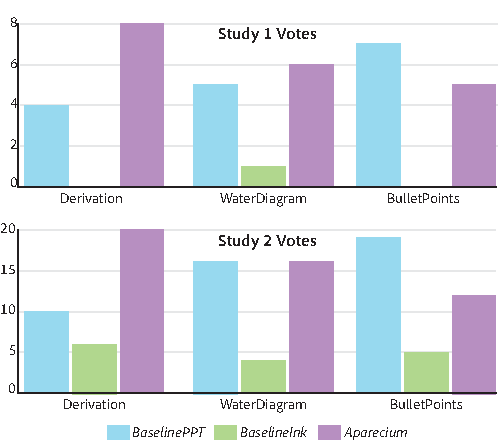
\includegraphics[width=1\columnwidth]{figures/studyVotes}
        \caption{Preferred tool/presentation for each content type.}
\label{fig:votes}
\end{figure}

\textbf{For presentation delivery, \interface\ involves comparable effort to BaslinePPT and less effort than BaselineInk.}\\
%{Kruskall-Walis chi squared: 4.044, p = 0.13}
%Presenters found it easiest to deliver the presentation using BaselinePPT, followed by our interface, and then BaselineInk. 
%
%The difference between BaselinePPT and our interface (Mann-Whitney U test: Z = 1.18, p = .24) was less significant than between that of BaselinePPT and BaselineInk (Z = -1.88, p = .06). \\
%
Regarding the ease of delivering presentations, BaselinePPT received slightly higher ratings than our interface. BaselineInk was rated the lowest by a larger margin. 
%
It is not surprising that BaselinePPT required the least effort. The only interaction presenters used was to press a single button to advance the slide animations. That said, when the animation involved more than a few steps, it was common for presenters to make mistakes. Three out of 12 participants forgot to advance the animation at the right time at least once, and only realized it at the next animation step. They had to either repeat the verbal explanation or quickly skip through the subsequent animations. In addition, two participants reported that they forgot to set up a desired animation step and only realized it during delivery. Several users suggested that having cues to help remember the animation would be beneficial $(U2, U7)$.

While presenters found inking in \interface\ straightforward, they noted that inking to reveal still required more effort than pushing a single button. Presenters seemed to prefer the path of minimum effort. For instance, with the exception of the math derivation content, they mostly used fast scribbling or strike-through gestures to reveal. As several presenters mentioned, this had the downside that the audience would initially see the scribbled ink strokes before the underlying pixels were revealed, which could potentially be distracting and aesthetically less pleasing. Some users suggested that they would prefer an even faster gesture such as clicking or circling to reveal large parts. On the other hand, they also expressed the idea that for the audience it could be better \textit{"to have the word appear after the inking instead of just after clicking like in powerpoint." (U1)} We discuss this tradeoff in more detail in the Limitations and Discussion section. %\val{I want to discuss the downsides of this path (e.g., less engaging for the audience, need setup (grouping of elements) but I don't want digress too much here.  What's a good phrase to signal the readers that we'll discuss this issue further later?}\wil{Maybe say that we discuss this tradeoff in more detail in Section X?}
%
In addition, users appreciated the automatic color selection for annotation and the modeless switching between revealing and inking. %\val{Should we mention here or in the Protocol, that space manipulation was not introduced the the participants for this study? Prefer in the protocol.}\wil{Agreed.}

As expected, BaselineInk required the most effort during delivery. Participants complained that drawing took away their attention from the content delivery. Since verbal explanations tend to be faster, there were periods of silence while the presenters were still drawing. In the Derivation presentation, three out of the four presenters who used BaselineInk ran out of space and had to use the margins or eraser. The one exception was a presenter who used the setup time to layout line numbers on the slide. In addition to these challenges, some users also complained about the specific difficulty of writing on a tablet. For example, the screen interface is not as smooth as paper \textit{(U1, U4, U6)} and operations such as switching to an eraser or a different color is tedious \textit{(U7, U9)}. 

\textbf{Presenters were most satisfied with the presentation quality of \interface\.}
Presenters were most satisfied with the presentations produced using \interface. As shown in Figure~\ref{fig:likert}, the distribution of ratings for BaselinePPT was slightly lower, while BaselineInk was rated the lowest.
%
%The difference between our interface and BaselinePPT was less significant (Z = -0.95, p = .34) than that between ours and BaselineInk (Z = -1.88, p = 0.06). 
%
This trend held overall, as well as for each individual content type.

The feedback we gathered was consistent with our preliminary, formative interviews. Participants were accustomed to the BaselinePPT style, but in many cases they thought it could be improved with finer grained animation \textit{(U1, U3, U4, U8, U11)}. They liked the \textit{"handwritten in real time effect" (U4)}   in \interface, as it made the presentation \textit{"more interactive and seem to require engagement " (U9)}. The main complaints about BaselineInk presentations were that the drawings looked \textit{"messy" (U7)} and \textit{"not professional enough" (U6)}, and that the pace was too slow.

\textbf{Tool preference depends on presentation content.}
The tool preferences of both the presenters and audience depended on the content type. (Figure~\ref{fig:votes})
%
In Study 1, we asked presenters to choose which interface they would prefer to use for each content type.
%
For Derivation, presenters preferred  \interface\ (8/12) and then BaslineInk (4/12). For WaterDiagram, \interface\ (6/12) and BaslinePPT(5/12) were comparable choices. Similarly for BulletPoints, BaselinePPT (7/12) and \interface\ (5/12) were preferred.
%

In Study 2, we asked audiences which presentation was most engaging. For Derivation, the majority of audiences preferred \interface\ (20/36) followed by BaselinePPT (10/36) and then BaselineInk (6/36). For WaterDiagram, \interface\ (16/36) and BaselinePPT (16/36) were comparable. For BulletPoints audiences preferred BaselinePPT (19/36) and then \interface\ (12/36).
%
These findings confirm our intuition that fine-grained control of pace is most important for presenting sequential processes, especially for writing out text or equations (Derivation). In the case of the WaterDiagram, it was easy to achieve similar sized steps using BaselinePPT and \interface. The fact that the WaterDiagram slide consists mainly of images rather than text may have affected the users choice as well (see discussion about different ways to reveal). %\val{Here, or in a separate discussion, I want to bring up the observation that for Derivation, people used slow inking, but for WaterDiagram or BulletPoints, people used scribbling (even for revealing simple images such as clouds). There could be many reasons. e.g., presenter laziness; it's more difficult to draw the contour of an image; the image doesn't require much description, so it's not appropriate to take much time to draw. Should we talk about this in discussion section? It seems to lead to questions we can't answer here but rather interesting topics for future work. For example, if the presenters actually drew the contours of the image in the WaterDiagram, would audience preference be different? Is there a different "best revealing strategy" for different content type? Should we allow lasso for some types of contents? etc.} \wil{Maybe here we can say that the elements in WaterDiagram point out some potential limitations of our current reveal interactions (assuming we can refer to specific examples in the study where people seemed to have trouble revealing elements) and that we believe these could be addressed with extensions to our method, which we discuss more in future work.}
%
For simple lists and images (BulletPoint), BaselinePPT provided an appropriate pace and aesthetics.

%\wil{Given that the overall message from the study results is pretty positive (generally easier for both preparation and delivery, and produces preferred results for some common content types), it would be nice to summarize this somewhere. Maybe as part of conclusions?} 

